% !TEX root = ../main.tex

\section{Experimental Results}
\label{sec:orgc23a664}

We show results on four different datasets, moviePosters, cancerHallmarks, chemicalExposure and Arxiv2020. Note that for the two medical datasets cancerHallmarks and chemicalExposure, information is a lot more sparse, we thus set the evaluation metrics threshold at 0.05 and train for 500 epochs until reaching convergence. 

In general, we observe that sigmoidF1 performs better on most metrics and across different datasets. In particular, sigmoidF1 always outperforms other losses on our metric of focus (weightedF1) and its non-weighted counterpart (microF1). On moviePosters and Arxiv2020, we observe higher scores on all but the precision metric. On the smaller chemicalExposure and cancerHallmarks datasets, macroSoftF1 delivers good results for macroF1 and precision and sigmoidF1 leads to higher results in the reminder of the metrics. Note that countrary to sigmoidF1, macroSoftF1 can be particularly performent without requiring hyperparameter tuning.

FocalLoss, which is specifically tailored for sparse data, does not perform well here, esxcept for precision on moviePosters. This can be explained by the fact that focal loss is designed for multiclass unilabel problems. Across Tables \ref{tab:chemicalExposure, tab:moviePosters, tab:arxiv2020, tab:cancerHallmarks} we see that the smooth sigmoidF1 outperforms other existing losses.

\todo{change to percentage & change order of metrics}

\begin{table}[htbp]
  \caption{Movie posters (CNN). \mdr{Explain what we see.}}
  \label{tab:moviePosters}
\centering
\begin{tabular}{l ccccc}
\toprule 
Loss  & \rotatebox{90}{macroF1 @ 0.5} & \rotatebox{90}{microF1 @ 0.5} & \rotatebox{90}{weightedF1 @ 0.5} & \rotatebox{90}{Precision @ 0.5} & \rotatebox{90}{Recall @ 0.5}\\ 
\midrule
$\mathcal{L}_{\text {CE}}$ & 0.051 & 0.186 & 0.149 & 0.090 & 0.042 \\
$\mathcal{L}_{\text {FL}}$ & 0.055 & 0.192 & 0.154 & 0.115 & – \\
% $\mathcal{L}_{\text {CE+N}}$ & 0 & 0 & 0 & 0 & 0 \\
$\mathcal{L}_{\text {macroSoftF1}}$ & 0.136 & 0.207 & 0.243 & \textbf{0.105} & 0.190 \\
$\mathcal{L}_{\text {sigmoidF1}}$ & \textbf{0.158} & \textbf{0.224} & \textbf{0.300} & 0.104 & \textbf{0.557} \\ % run aa424792a57e4208ad1805cd6e63f8e6
\bottomrule
\end{tabular}
\end{table}


\begin{table}[htbp]
  \caption{Arxiv (distillBERT 2020), frozen pretrained weights 100 epochs, min-label-thresh: 1000}
  \label{tab:arxiv2020}  
\centering
\begin{tabular}{l ccccc}
\toprule
Loss  & \rotatebox{90}{macroF1 @ 0.5} & \rotatebox{90}{microF1 @ 0.5} & \rotatebox{90}{weightedF1 @ 0.5} & \rotatebox{90}{Precision @ 0.5} & \rotatebox{90}{Recall @ 0.5}\\ 
\midrule
$\mathcal{L}_{\text {CE}}$ & 0.093 & 0.106 & 0.106 & 0.096 & – \\ % Run 71ef078f975649d5b3d897e504bc638b
$\mathcal{L}_{\text {FL}}$ & 0.008 & 0.011 & 0.009 & 0.054 & 0.954 \\
% $\mathcal{L}_{\text {CE+N}}$ & 0 & 0 & 0 & 0 & 0 \\
$\mathcal{L}_{\text {macroSoftF1}}$ & 0.077 & 0.088 & 0.087 & \textbf{0.100} & – \\ % run 405a6e6851e84a89a82313251a7a36e8 (18-19 jan)
$\mathcal{L}_{\text {sigmoidF1}}$ & \textbf{0.093} & \textbf{0.106} & \textbf{0.106} & 0.096 & \textbf{–} \\ % run bd478ca55eb64cc78d9ad0f25accce35 (18-19 jan)
\bottomrule
\end{tabular}
\end{table}

\begin{table}[htbp]
  \caption{Cancer Hallmarks}
  \label{tab:cancerHallmarks}
\centering
\begin{tabular}{l ccccc}
\toprule 
Loss  & \rotatebox{90}{macroF1 @ 0.05} & \rotatebox{90}{microF1 @ 0.05} & \rotatebox{90}{weightedF1 @ 0.05} & \rotatebox{90}{Precision @ 0.05} & \rotatebox{90}{Recall @ 0.05}\\ 
\midrule
$\mathcal{L}_{\text {CE}}$ & 0.0 & 0.0 & 0.0 & 0.0 & 0.0 \\ 
$\mathcal{L}_{\text {FL}}$ & 0.044 & 0.190 & 0.108 & 0.071 & 0.055 \\
% $\mathcal{L}_{\text {CE+N}}$ & 0 & 0 & 0 & 0 & 0 \\
$\mathcal{L}_{\text {macroSoftF1}}$ & \textbf{0.098} & 0.176 & 0.170 & \textbf{0.089} & 0.131 \\
$\mathcal{L}_{\text {sigmoidF1}}$ & 0.095 & \textbf{0.313} & \textbf{0.202} & 0.059 & \textbf{0.264} \\ % run e145056949424b02bfc83cc57af38374
\bottomrule
\end{tabular}
\end{table}


\begin{table}[htbp]
  \caption{Chemical Exposure}
  \label{tab:chemicalExposure}
\centering
\begin{tabular}{l ccccc}
\toprule
Loss  & \rotatebox{90}{macroF1 @ 0.05} & \rotatebox{90}{microF1 @ 0.05} & \rotatebox{90}{weightedF1 @ 0.05} & \rotatebox{90}{Precision @ 0.05} & \rotatebox{90}{Recall @ 0.05}\\ 
\midrule
$\mathcal{L}_{\text {CE}}$ & 0.012 & 0.058 & 0.051 & 0.047 & 0.007 \\ % Run 71ef078f975649d5b3d897e504bc638b
$\mathcal{L}_{\text {FL}}$ & 0.0934 & 0.348 & 0.268 & 0.130 & 0.091 \\
$\mathcal{L}_{\text {macroSoftF1}}$ & \textbf{0.133} & 0.194 & 0.218 & \textbf{0.155} & 0.138 \\ % run 405a6e6851e84a89a82313251a7a36e8 (18-19 jan)
$\mathcal{L}_{\text {sigmoidF1}}$ & 0.113 & \textbf{0.432} & \textbf{0.319} & 0.091 & \textbf{0.188} \\ % run a30825efe9c94a24bc46a9c71a5f8646 E: 0.5 S: 0.6
\bottomrule
\end{tabular}
\end{table}


\subsection{Sensitivity Analysis}

\begin{figure}[htbp]
\centering
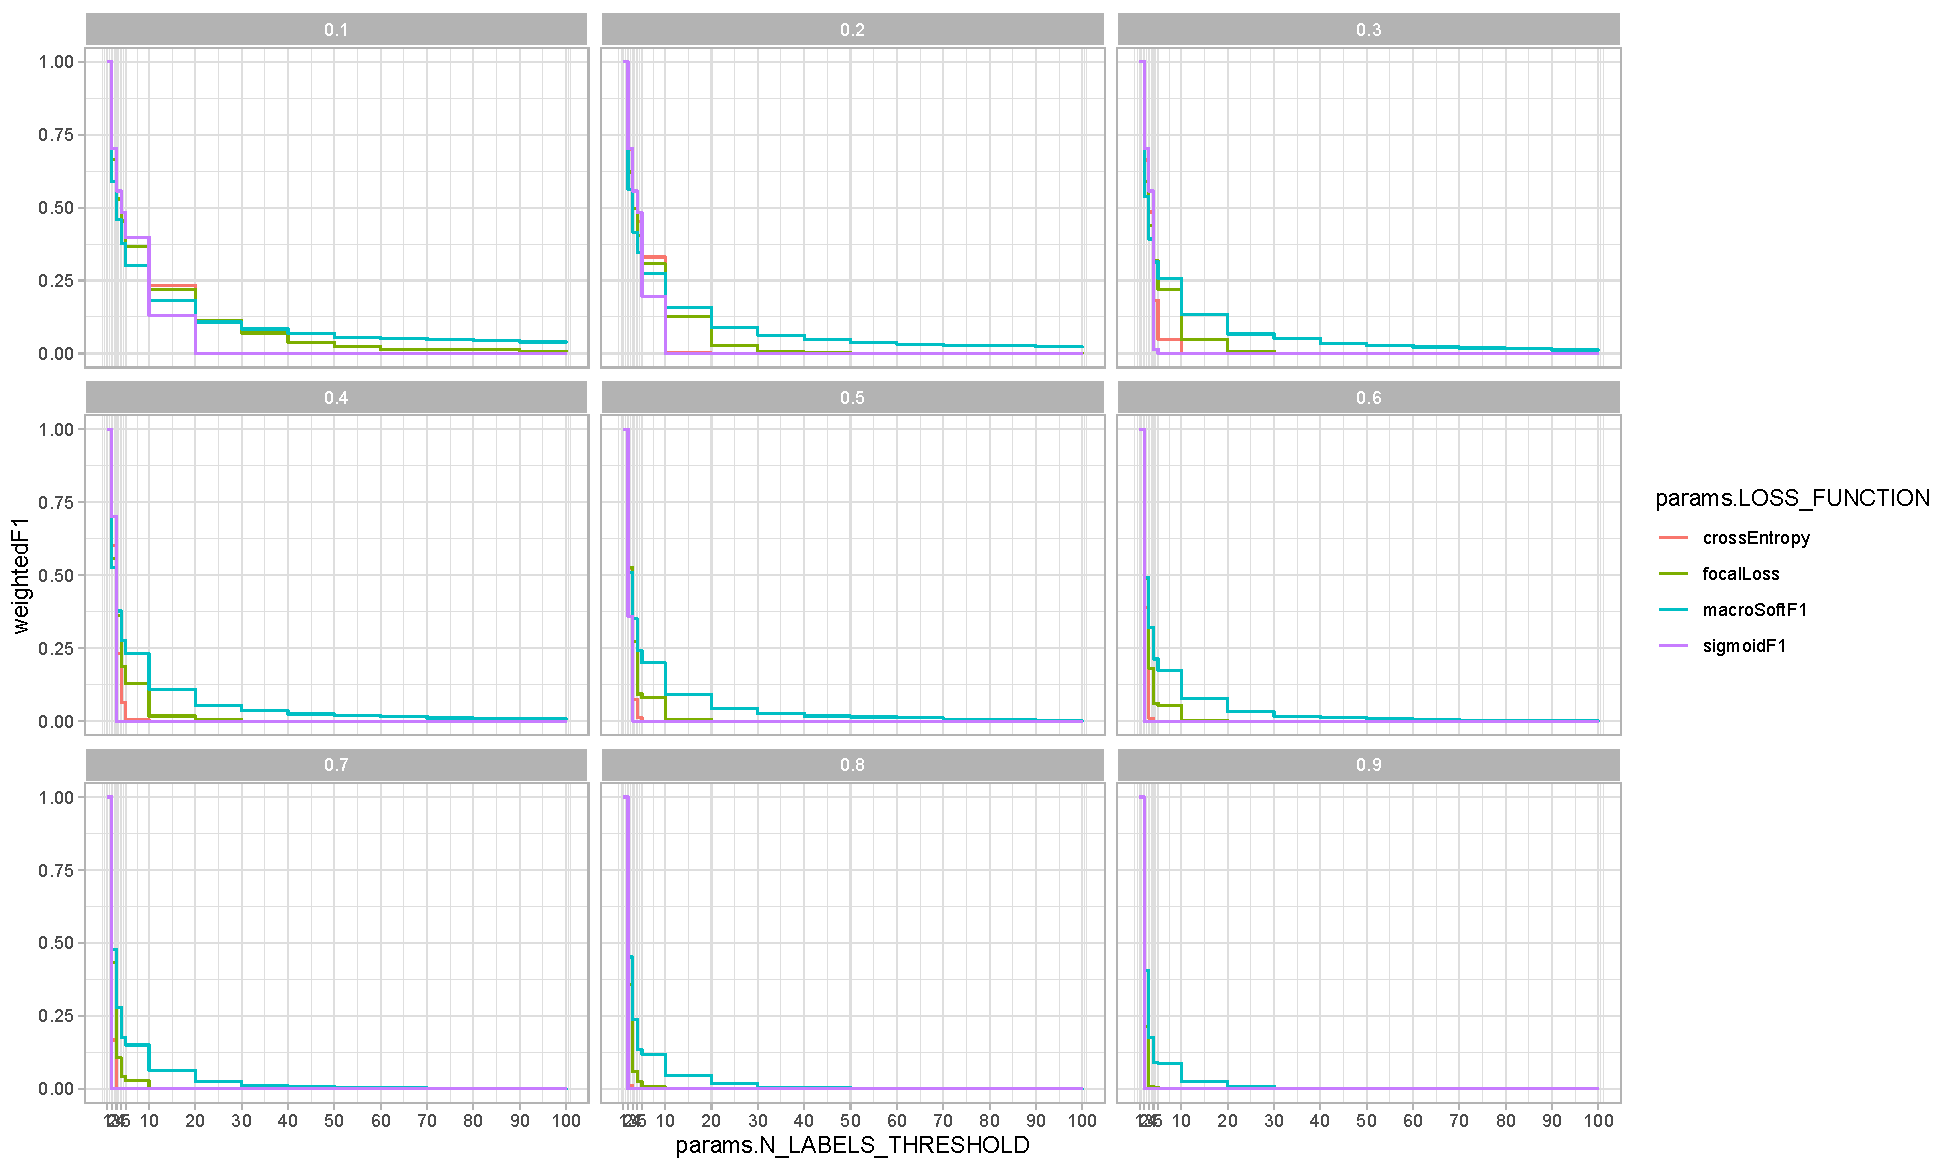
\includegraphics[width=.9\linewidth]{./images/ablation.pdf}
\caption{\label{fig:etaBeta}
weighted F1 score at different threshold (x axis) and for different values of Eta and Beta. Dots connected with a line are from the same experiment.}
\end{figure}




\subsection{Ablation Study - Arxiv2020}

We performed an analysis of sensitivity to different amount of labels. For this, the irrelevance threshold (see definition in Section \ref{sec:orgb44ba25}) $t$ was set to the values 0, 10, 100 and 1000. This time, results are shown with dichotomization thresholds of 0.1 to 0.9. \todo{see if keep it}

\todo{sensitivity to hyperparametertuning plot}

\begin{figure}[htbp]
\centering
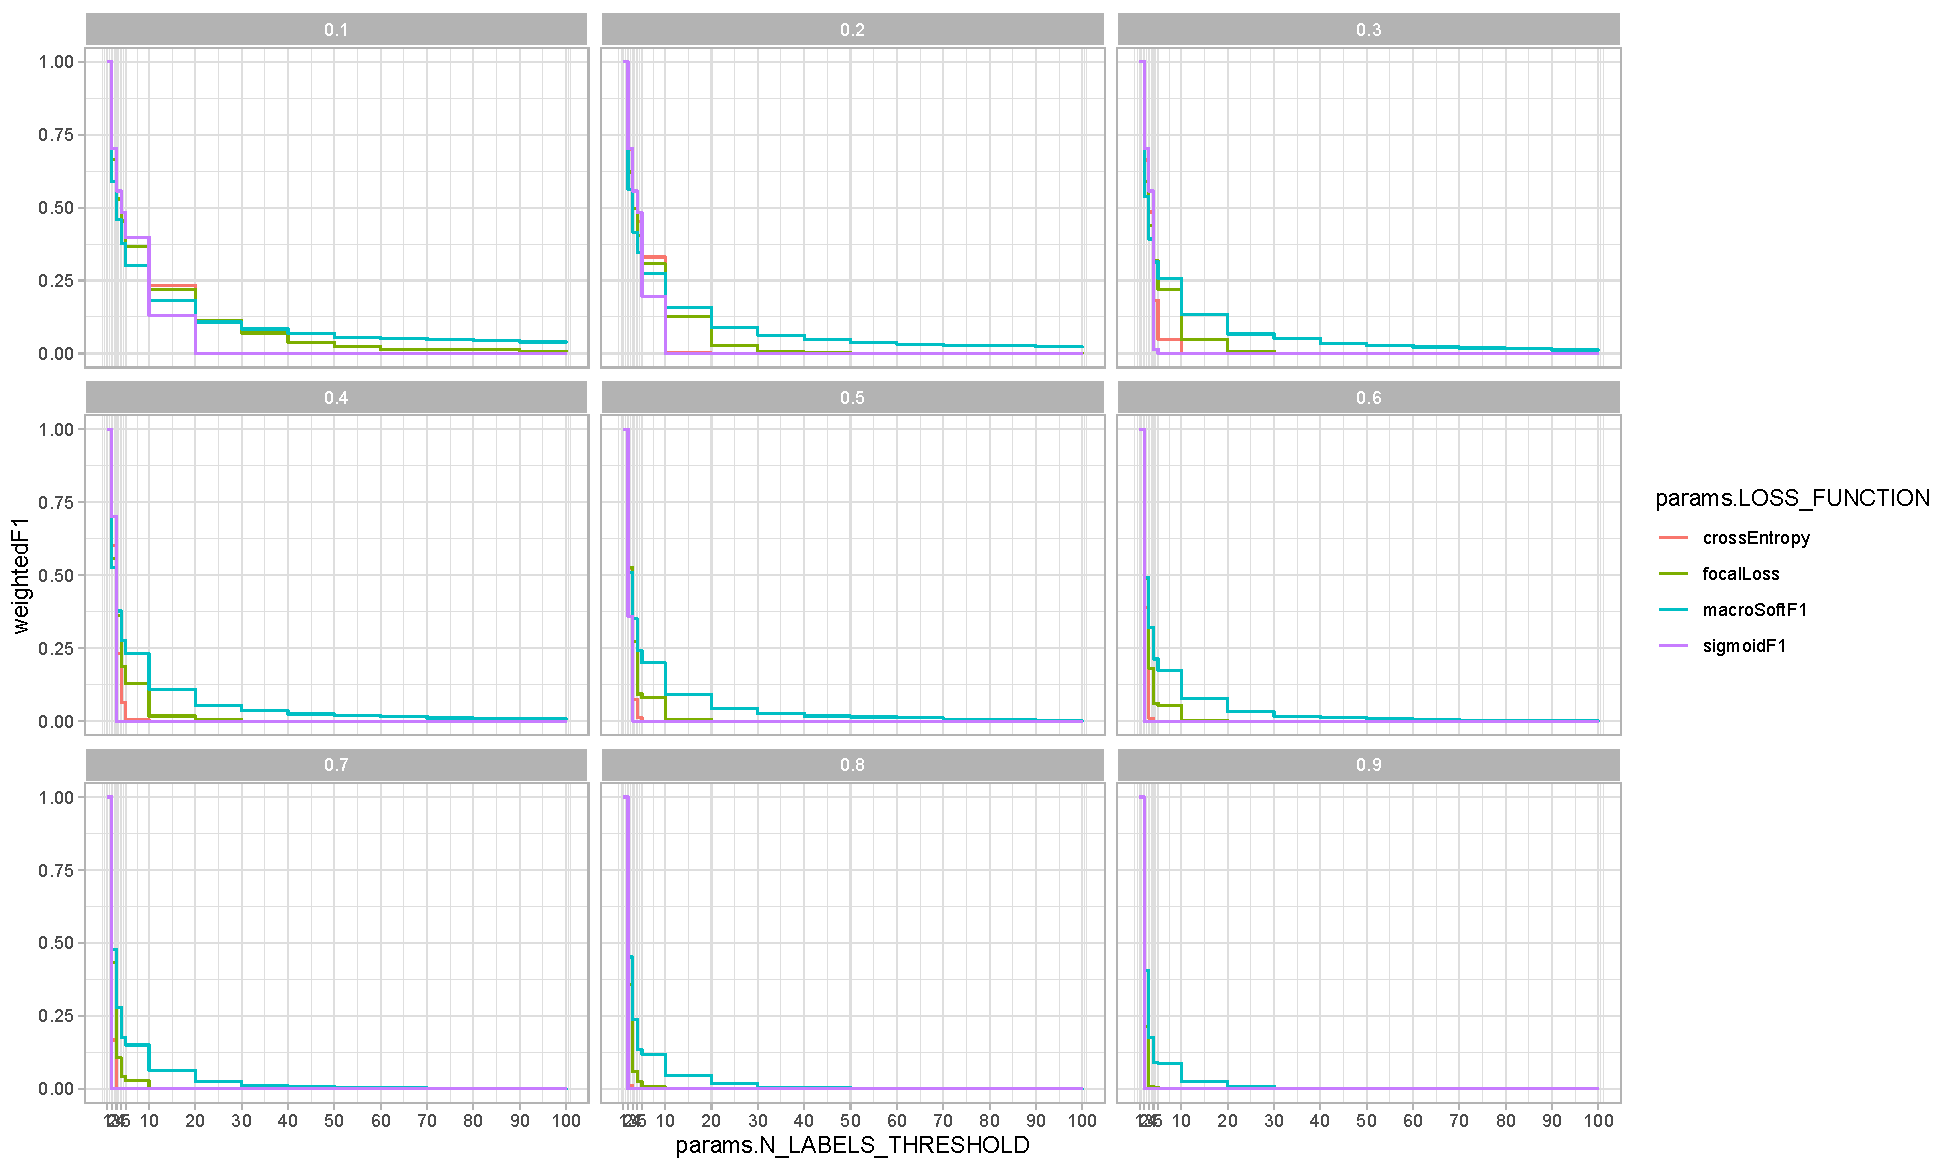
\includegraphics[width=.9\linewidth]{./images/ablation.pdf}
\caption{\label{fig:ablation}
Sigmoid function with different values for $\beta$ (steepness) \& $\eta$ (offset)}
\end{figure}




%%% Local Variables:
%%% mode: latex
%%% TeX-master: "../main"
%%% End:
